
\chapter{Galois Groups and the Main Theorem of Galois Theory}
\label{cha:galois-groups-galois}

We now come to a central definition of this course. 

\begin{definition}
  \label{def:2}
  If $E ⊇F$ is an extension of fields, an automorphism $σ: E → E$ that satisfies $σ(a) = a$ for each $a ∈ F$ is said to \emph{fix} $F$ and it is called an \emph{$F$-automorphism}.  The set of $F$-automorphisms are, together with composition a group. It is called the \emph{Galois group} of the extension $E ⊇F$ and we denote it by $\gal(E:F)$.
\end{definition}

The next lemma is simple to prove, but very helpful in understanding the Galois group.

\begin{lemma}
  \label{lem:2}
  Let $E ⊇F$  be a field extension, $f(x) ∈ F[x]$, $τ ∈ \gal(E:F)$ and $u ∈ E$. Then $τ(f(u)) = f(τ(u))$. In particular, if $u$ is a root of $f$, then so is $τ(u)$. 
\end{lemma}
\begin{proof}
  Let $f(x)  = a_0 + a_1x + \cdots + a_n x^n ∈F[x]$, then
  \begin{eqnarray*}
    τ(f(u)) & = & τ (a_0 + a_1u + \cdots + a_n u^n) \\
            & = & τ (a_0) + τ(a_1u)  + \cdots + τ(a_n u^n) \\
            & = & τ (a_0) + τ(a_1)τ(u)  + \cdots + τ(a_n) τ (u)^n \\
            & = &  a_0 + a_1τ(u)  + \cdots + a_n τ (u)^n,
  \end{eqnarray*}
  where the  second and third row follow  from the homomorphism property of $τ$ and the last row from the fact that $τ$ fixes $F$. 
\end{proof}

\begin{theorem}
  \label{thr:17}
  Let $F(u) ⊇F$ be a simple and finite extension, let $p(x) ∈ F[x]$ be the minimal polynomial of $u$ and let $u=u_1, u_2,\dots,u_k$ be the other roots of $p(x)$ that are contained in $F(u)$. Then
  \begin{displaymath}
    \gal(F(u) :F) = \{ σ_1,\dots,σ_k\} 
  \end{displaymath}
  where $σ_i: F(u) → F(u)$ is the unique $F$-automorphism that maps $u$ to $u_i$. 
\end{theorem}

\begin{proof}
   Suppose that the degree of $p(x)$ is $n$.
  
  Let $τ ∈ \gal(E:F)$ be given. Lemma~\ref{lem:2} shows that $τ(u) = u_i$ for some $i∈ \{1,\dots,k\}$ must hold. Also, each element of $F(u)$ is of the form $f(u)$ with $f(x) ∈ F[x]$. This shows that $τ$ is uniquely specified by the image of $u$, which is another root of $p(x)$ in $F(u)$.

  On the other hand, $F(u) = F(u_i)$ for each $i=1,\dots,k$. An element of $F(u)$ is of the form $a_0+ a_1 u + \cdots + a_{n-1} u^{n-1}$ with $a_i ∈F$. The mapping  $τ_i:F(u)→F(u)$ with $a_0+ a_1 u + \cdots + a_{n-1} u^{n-1} ↦ a_0+ a_1 u_i + \cdots + a_{n-1} u_i^{n-1}$  is an $F$-automorphism which maps $u$ to $u_i$. 
\end{proof}




Equipped with this knowledge, we can start determining some Galois groups. 

\begin{example}
  \label{exe:2}
  Let us determine $\gal(ℂ:ℝ)$. Since $ℂ = ℝ(i)$ and $-i$ is the other
  root of the minimal polynomial $x^2+1$ of $i$, we understand that
  $\gal(ℂ:ℝ) =\{ id, γ\}$, where $γ$ is the complex conjugation
  automorphism.
\end{example}


\begin{example}
  \label{exe:3}
  Let $u = \sqrt[3]{2}$ and consider the extension $ℚ(u) ⊇ ℚ$. The minimal polynomial of $u$ is $x^3 -2$. The other roots of this polynomial are $w u$ and $w^2 u$ with $w =e^{2πi/3}$. These other roots are not in $ℝ$. Therefore, we conclude that $\gal( ℚ(u) : ℚ) = \{id \}$. 
\end{example}


\begin{example}
  \label{exe:4}
  Let $ u = e^{2πi/p}$, where $p$ is a prime number and consider $ℚ(u) ⊇ℚ$. The minimal polynomial of $u$ is $1+ x + \cdots +  x^{p-1}$, the $p$-th cyclotomic polynomial. The other roots of this polynomial are $u^2,\dots,u^{p-1}$ and they are all different. Thus, by Theorem~\ref{thr:17}, $|\gal(ℚ(u):ℚ)| = p-1$. Furthermore, there exists an element $τ ∈ \gal(ℚ(u):ℚ)$ with $τ(u) = u^m$, where $m$ is a generator of $ℤ_p^*$. Clearly,  $τ^i(u) = u^{m^i} = u^{m^i \pmod{p}}$. This proves that the order of $τ$ as an element of $\gal(ℚ(u):ℚ)$ is $p-1$ and thus that $\gal(ℚ(u):ℚ) ≅ C_{p-1}$. 

\end{example}



\begin{example}
  \label{exe:5}
  Let $E = \mathrm{GF}(p^n) ⊇ ℤ_p$ be an extension of degree $n$ of $ℤ_p$. We show that $\gal(E:F) ≅ C_n$. To this end, denote   $F = ℤ_p$ and since $E$ is cyclic, we have $E = F(u)$. The minimal polynomial $p(x) ∈ F[x]$ has degree $n$ and with Theorem~\ref{thr:17} $|\gal(E:F)| ≤ n$.  Consider the Frobenius automorphism
  \begin{displaymath}
    φ(x) = x^p, \text{ for each } x ∈E. 
  \end{displaymath}
  One has  $φ^i(x) = x^{p^i}$
 Therefore, if the order of $φ$ is $k$, then each element of $E$ satisfies $x^{p^k} -x = 0$. Therefore, the order of $φ$ is $n$ and this shows that $\gal(E:F) ≅ C_n$. 
\end{example}



\begin{theorem}
  \label{thr:18}
  Let $E ⊇F$ be a finite extension, $E = F(u_1,\dots,u_n)$ and let $p_i(x) ∈ F[x]$ be the minimal polynomial of $u_i$. If $τ ∈ \gal(E:F)$, then
  \begin{enumerate}[i)] 
  \item $τ$ is uniquely determined by the choice of $τ(u_1),\dots,τ(u_n)$
  \item $τ(u_i)$ is a root of $p_i(x)$.  
  \end{enumerate}
\end{theorem}

Recall the group $D_n$. It is generated by an element $a$ of order $n$, an element $b≠a$ or order $2$ and one has $aba = b$. $D_n$ has $2n$  elements, namely 
\begin{displaymath}
  1,a,a^2,\dots,a^{n-1}, b,ba,\dots, ba^{n-1}. 
\end{displaymath}


\begin{example}
  \label{exe:6}
  Let $E$ denote the splitting field of $x^3 -2$ over $ℚ$. We show that $\gal(E:ℚ) ≅ D_3$.  We denote $\gal(E:ℚ)$ by $G$. Let $u = \sqrt[3]{2}$ and $w = e^{2πi/3}$. % Clearly, $[E:ℚ] = 6$ because $ℚ(u) ⊆ ℝ$,  $[ℚ(u):ℚ]=3$ and $6 = 3! ≥ [E:ℚ] = [E:ℚ(u)][ℚ(u):ℚ]$.

  Let $τ$ be a $ℚ$-automorphism. Theorem~\ref{thr:18} shows that $τ(u) ∈ \{ u,uw,uw^2\}$ and $τ(w) ∈ \{ w, w^2\}$ and thus that $|G| ≤ 6$. This also follows from the fact that $[E:ℚ] ≤ 3⋅2$ and that $E$ is a primitive extension. We apply Theorem~\ref{thr:13}.

\begin{displaymath}
  \begin{CD}
    E=ℚ(u,w) @>σ>> ℚ(uw,w)=E \\
    @AAA     @AAA \\
    ℚ(u) @>σ_0 >>ℚ(uw) \\
    @AAA     @AAA \\
     ℚ @>id >>ℚ
  \end{CD}
\end{displaymath}
and obtain a $ℚ$-automorphism $σ$ with $σ(u) = uw$ and $σ(w) = w$. The order of this $σ$ is three. Similarly, we can construct a $ℚ$-automoprhism $τ$ with $τ(u) = u$ and $τ(w) = w^2$. The order of $τ$ is $2$ and $στσ = τ$.  


  
\end{example}


A group $G$ of permutations on a set $X$ is to \emph{act transitively} on $X$ if for each $u,v ∈X$ there exists $τ ∈G$ with $τ(u) = v$.

\begin{theorem}
  \label{thr:19}
  Let $E ⊇F$ be the splitting field of a polynomial $f(x) ∈ F[x]$ and let $X$ denote the set of roots of $f(x)$ in $E$. Then
  \begin{enumerate}[i)] 
  \item $\gal(E:F)$ is isomorphic to a subgroup of $S_X$.\label{item:1}
  \item If $f(x)$ is irreducible, then $\gal(E:F)$ acts transitively on $X$.\label{item:2}
  \item If $f(x)$ is separable, and if $\gal(E:F)$ acts transitively on $X$, then $f(x)$ is irreducible.  \label{item:3}
  \end{enumerate}
\end{theorem}

\begin{proof}
  \ref{item:1}) is clear. Let $u,w$ be roots of $f(x)$, then $F(u) ≅F(w)$ with an $F$-automorphism that maps $u$ to $w$. By Theorem~\ref{thr:13} this can be extended to an $F$ automorphism of $E$. This implies~\ref{item:2}). To show~\ref{item:3}) we suppose that $f = gh$ with $\deg(f),\deg(g)≥1$. Let $g(u) = h(v) = 0$ for some $u,v ∈E$. Since $\gal(E:F)$ acts transitively on $X$ there exists a $τ ∈ \gal(E:F)$ with $τ(u) = v$ and thus $0=τ(g(u)) = g(τ(u))=g(v)$ which contradicts that $f$ has no repeated roots.

  
\end{proof}


\section{Normal extensions}
\label{sec:normal-extensions}



\begin{definition}
  \label{def:3}
  A field extension $E ⊇F$ is called \emph{normal extension} if every irreducible polynomial in $F[x]$ that has a root in $E$ splits into linear factors in $E[x]$.
\end{definition}


\begin{example}
  \label{exe:7}
  $ℂ⊇ℝ$ is a normal extension. The extension $ℚ(\sqrt[3]{2}) ⊇ ℚ$ is not normal, as $x^3 - 2$ does not split into linear factors.  
\end{example}


\begin{theorem}
  \label{thr:20}
  An extension $E ⊇ F$ is normal and finite if and only if it is the splitting field of a polynomial over $F$. 
\end{theorem}

\begin{figure}
  \centering
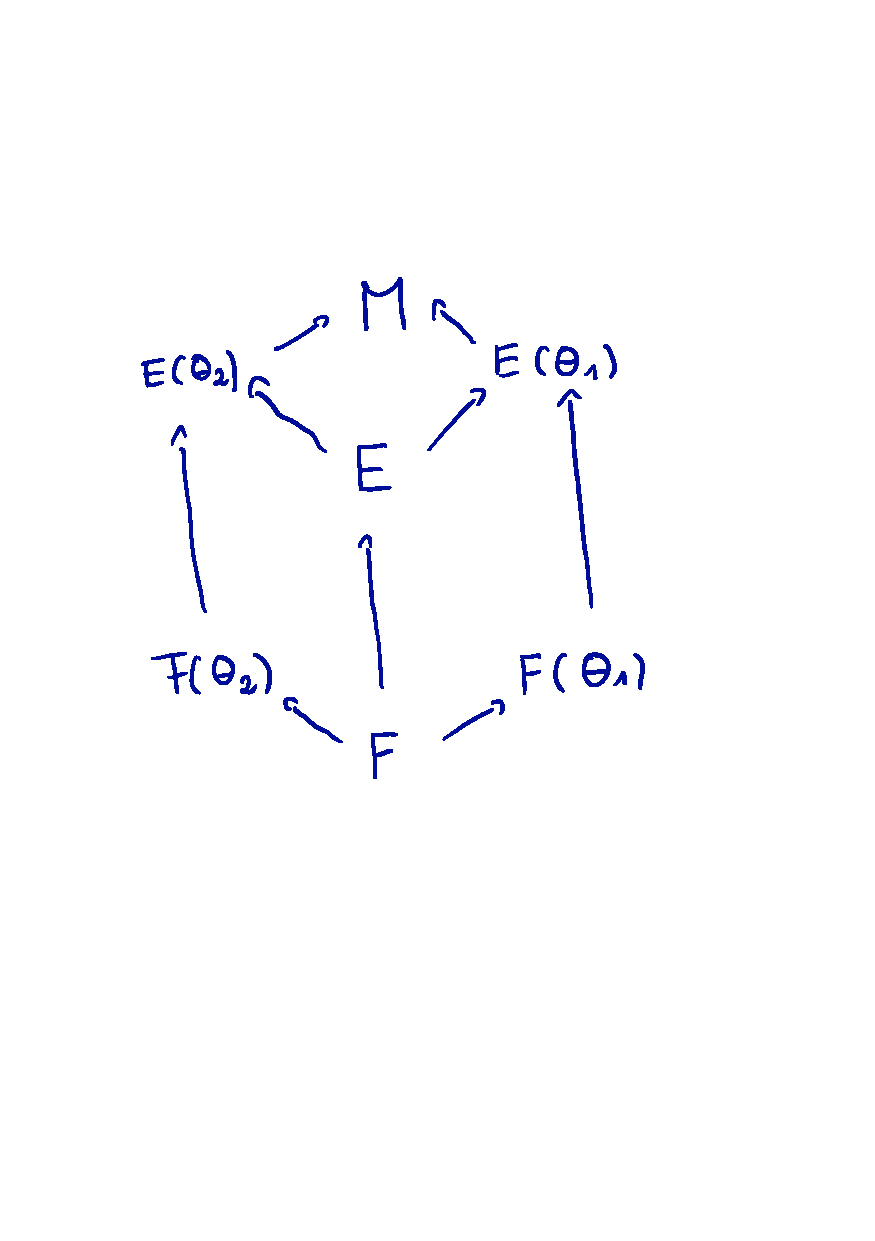
\includegraphics{normal.pdf}  
  \caption{Illustration of the proof of Theorem~\ref{thr:20}}
  \label{fig:1}
\end{figure}



\begin{proof}
  Suppose that $E ⊇ F$ is normal and finite. Then $E = F(u_1,\dots,u_k)$. Each minimal polynomial $p_i(x) ∈ F[x]$ splits into linear factors over $E$, one factor being $(x  - u_i)$. This shows that $E$ is the splitting field of $p_1(x) \cdots p_k(x)$.

  For the converse we assume that $E$ is the splitting field of $f(x) ∈F[x]$ and let $p(x) ∈ F[x]$ be an irreducible polynomial that has a root $θ_1$ in $E$.  Let $M$ be a splitting field of $p(x)$ over $E$ and let  $θ_2$ be another root of $p(x)$ in $M$. The fields $F(θ_1)$ and $F(θ_2)$ are isomorphic. The fields $E(θ_1)$ and $E(θ_2)$ are splitting fields of $f(x)$ over $F(θ_1)$ and $F(θ_2)$ respectively. Theorem~\ref{thr:13} shows that the extensions $E(θ_1)⊇F(θ_1)$ and $E(θ_2)⊇F(θ_2)$  are isomorphic and have the same degree. One has
  \begin{displaymath}
    [E(θ_1):F]  =   [E(θ_1):F(θ_1) ] ⋅ [F(θ_1) :F]  
  \end{displaymath}
  and
  \begin{displaymath}
        [E(θ_2):F]  =   [E(θ_2):F(θ_2) ] ⋅ [F(θ_2) :F]. 
  \end{displaymath}
   which proves, $ [E(θ_1):F ] = [E(θ_2):F ]$. On the other hand, one has
   \begin{displaymath}
      [E(θ_1):F ]  =   [E(θ_1):E ] ⋅ [E :F] 
    \end{displaymath}
    and
    \begin{displaymath}
      [E(θ_2):F ]  =   [E(θ_2):E] ⋅ [E :F] 
    \end{displaymath}
  which shows that $[E(θ_1):E ] =[E(θ_2):E]$ and thus that also $θ_2 ∈ E$. 
\end{proof}

Theorem~\ref{thr:20} has a very important consequence. Let $E ⊇F$ be a finite  normal and separable extension. Then, it is a primitive extension  $E = F(u)$ by Theorem~\ref{thr:16}. Furthermore, if $p(x)∈F[x]$ is the minimal polynomial of $u$, then $p(x)$ splits into linear factors in $E$
\begin{displaymath}
  p(x) = (x-u_1) \cdots (x-u_n),
\end{displaymath}
where $u_1=u$ and $u_2,\dots,u_n$ are the other roots pf $p(x)$. 
Theorem~\ref{thr:17} tells us that  $\gal(E:F) = \{ τ_1,\dots,τ_n\}$ where $τ_i$ is the unique $F$-automorphism that maps $u$ to $u_i$. Thus we fully understand the Galois group of a finite normal and separable field extensions, once we get a hold on the primitive element, its minimal polynomial and the other roots of the minimal polynomial as $F$-linear combinations of $1,u,\dots,u^{n-1}$. We will elaborate on this further. 

\section{Group characters and Dedekind's lemma}
\label{sec:group-char-dedek}

\begin{definition}
  \label{def:4}
  Let $G$ be a group and $E$ a field. A group homomorphism $σ:G → E^*$ is called a \emph{character} of $G$ in $E$. A set $\{σ_1,\dots,σ_n\}$ of characters is called \emph{independent'} if for $e_1,\dots, e_n ∈ E$
  \begin{displaymath}
    e_1 σ_1(g) + \cdots + e_n σ_n(g) = 0 \, \text{ for each } g ∈ G 
  \end{displaymath}
  implies $e_1=\cdots=e_n=0$. 
\end{definition}


\begin{lemma}[Dedekind's Lemma]
  \label{lem:3}
  A finite set of distinct characters of a group $G$ in a field $E$ is independent. 
\end{lemma}

\begin{proof}
  Let $\{σ_1,\dots,σ_n\}$ be a set of distinct characters of $G$ in $E$ for which the assertion is to be shown. We proceed by induction on $n$. For $n=1$ one observes that if $u_1 σ_1(g) = 0$ for each $g ∈G$, then $u_1=0$ since $σ_1(g) ≠0$ for each $g ∈G$.

  For  $n>1$, let $e_1,\dots,e_n ∈E$ with
  \begin{equation}
    \label{eq:15}
   e_1  σ_1(g) + \cdots + e_n  σ_n(g) = 0 \text{ for each } g ∈G.     
  \end{equation}
 We need to show that all $e_i$ are zero. If one $e_i$ is zero, then, by the induction hypothesis,  all others are zero as well. Assume that that all $e_i$ are non-zero. For  $h ∈G$ one has $σ_i(h⋅ g) = σ_i(h) ⋅σ_i(g)$  and clearly
 \begin{equation}
   \label{eq:16}
   e_1  σ_1(h) σ_1(g) + \cdots + e_n  σ_n(h) σ_n(g) = 0 \text{ for each } g ∈G.
 \end{equation}
%
By multiplying~\eqref{eq:15} with $σ_1(h)$ and subtracting  equation~\eqref{eq:16} from the result one obtains 
\begin{displaymath}
   e_2  (σ_1(h) - σ_2(h))   σ_2(g) + \cdots + e_n  (σ_1(h) - σ_n(h))  σ_n(g) = 0 \text{ for each } g ∈G.
 \end{displaymath}
 By the induction hypothesis and the fact that each $e_i$ is non-zero, this means that
 \begin{displaymath}
    (σ_1(h) - σ_i(h)) \, ∀ i∈\{2,\dots,n\}, \ h ∈G 
  \end{displaymath}
  and thus that the characters are all equal, contrary to the assumption that they are distinct.
\end{proof}


\begin{theorem}
  \label{thr:21}
  Let $E ⊇F$ be a finite field extension and denote $\gal(E:F)$ by $G$. One has
  \begin{displaymath}
    |G| ≤ [E:F]. 
  \end{displaymath}
\end{theorem}
\begin{proof}
  Let $[E:F] = n$, $v_1,\dots,v_n ∈E$ be an $F$-basis of $E$ and suppose that there are $n+1$ distinct $F$-automorphisms $σ_0,\dots,σ_n ∈ G$. These are also characters from the group $E^*$ into $E$ and this means that they are independent. Consider the matrix
  \begin{displaymath}
    A =
    \begin{pmatrix}
      σ_0(v_1) & σ_1(v_1) &  \cdots & σ_n(v_1) \\
      σ_0(v_2) & σ_1(v_2) &  \cdots & σ_n(v_2) \\
      \vdots &           &         & \vdots \\
       σ_0(v_n) & σ_1(v_n) &  \cdots & σ_n(v_n) \\
    \end{pmatrix} ∈ E^{n ×n+1}. 
  \end{displaymath}
  There exists a nonzero vector $(x_0,\dots,x_{n})^T ∈E^{n+1}$ which is in the kernel of this matrix. In particular, one has
  \begin{equation}
    \label{eq:17}
    y^T A x = 0 \text{ for each } y ∈ F^{n}. 
  \end{equation}
  The $σ_i$ are $F$-automorphisms and thus 
  \begin{displaymath}
    y^T A = \left( σ_0\left(∑_{i=1}^n y_i v_i\right), σ_1\left(∑_{i=1}^n y_i v_i\right), \dots, σ_1\left(∑_{i=1}^n y_i v_i\right) \right). 
  \end{displaymath}
  Since each element of $E$ is a linear combination of the $v_i$, this, together with~\eqref{eq:17} means that
  \begin{displaymath}
    x_0 σ_0(e)+ \cdots +  x_n σ_n(e) = 0 \text{ for each } e ∈ E. 
  \end{displaymath}
  This is a contradiction, since $x ≠ 0$ and the characters $σ_0,\dots,σ_n$ are independent. Therefore, the assertion follows. 
\end{proof}


Let $σ: E→E$ be a field automorphism. Let us consider the elements of $E$ that are \emph{fixed} by $σ$, i.e., those $e ∈E$ with $σ(e) = e$. These elements are a field, which is quickly verified: Suppose $a$ and $b≠0$ are fixed. Then
\begin{eqnarray*}
  σ(a-b) & = &  σ(a) - σ(b) = a-b\\
  σ(a/b) & = &  σ(a) / σ(b) = a/b.\\   
\end{eqnarray*}
Let $G$ be a group of automorphisms of $E$. The set of elements of $E$ that are fixed by each  $σ ∈G$ is a field, as it is the intersection of all fixed fields of the elements of $G$. We denote this field by $E_G$. 


\begin{theorem}[Dedekind-Artin Theorem]
  \label{thr:25}
  Let $E$ be a field and $G$ be a finite group of automorphisms of $E$, then $E ⊇ E_G$ is a finite extension and 
  \begin{displaymath}
    |G| = [E :E_G]. 
  \end{displaymath}
\end{theorem}
\begin{proof}
  Let $n = |G|$. Assume that there are $n+1$ $E_G$-linear independent elements $u_0,\dots,u_n$ of $E$. We will lead this assumption to a contradiction. This implies the statement, since $|G| ≤ |\gal(E: E_G)| ≤ [E :E_G]$, where the latter inequality is Theorem~\ref{thr:25}.

Consider the following set of $n$ linear equations in $n+1$ variables $x_0,\dots,x_n$
  \begin{equation}
    \label{eq:19}
    σ(u_0) x_0 + \dots +  σ(u_n) x_n = 0,  \, σ ∈G. 
  \end{equation}
This has a nontrivial solution in $E^{n+1}$ and among these solutions let $x^* ∈E^{n+1}$ be a nontrivial solution with  a minimal number $r+1$ of nonzero components. By re-labeling, we can assume that the first $r+1$ components of $x^*$ are non-zero. Furthermore, by multiplying $x^*$ with $1/x^*_0$, we can assume  $x^*_0=1$. This means that 
  \begin{equation}
    \label{eq:21}
     σ(u_0)  + σ(u_1) x^*_1 \dots +  σ(u_n) x^*_r = 0, \, σ ∈G
   \end{equation}
   holds. 
  Since the identity is contained in $G$, one has 
  \begin{equation}
    \label{eq:20}
    u_0 + u_1 x^*_1 + \dots + u_r x^*_r = 0
  \end{equation}
  which implies that one of the $x^*_i$ is not contained in the fixed-field $E_G$. Thus, there exists a $τ ∈ G$ with $τ(x^*_i)≠ x^*_i$. By applying $τ$ to~\eqref{eq:21} we obtain
  \begin{equation}
    \label{eq:22}
     τ(σ(u_0))  + τ(σ(u_1)) τ( x^*_1) + \dots +  τ(σ(u_n))τ( x^*_r) = 0, \, σ ∈G.
   \end{equation}
   and since $τ \circ σ$ runs through the entire group as well, we can re-write~\eqref{eq:22} as
   \begin{equation}
     \label{eq:23}
      σ(u_0)  + σ(u_1) τ( x^*_1) \dots +  σ(u_n) τ( x^*_r) = 0, \, σ ∈G.
    \end{equation}
    Subtracting~\eqref{eq:23} from~\eqref{eq:21} yields
    \begin{equation}
      \label{eq:24}
      σ(u_1) (x^*_1- τ(x^*_1)) +  \dots +  σ(u_n) (x^*_r - τ(x^*_r))= 0, \, σ ∈G.
    \end{equation}
    This is a nontrivial solution to~\eqref{eq:19} with fewer than $r+1$ nonzero components. Namely the solution $y^*$ with
    \begin{displaymath}
      y^*_i =
      \begin{cases}
        (x^*_i- τ(x^*_i)) & 1 ≤ i  ≤ r \\
        0 & \text{ otherwise.}
      \end{cases}
    \end{displaymath}
\end{proof}

\section{Galois extensions}
\label{sec:galois-extensions}


\begin{definition}
  \label{def:5}
  A field extension $E ⊇F$ is called a Galois extension, if $F = E_{\gal(E:F)}$. 
\end{definition}  


\begin{example}
  \label{exe:8}
  The extension $ℂ ⊇ ℝ$ is Galois, since the complex conjugate of any non-real complex number is different from that number. 
\end{example}
 
\begin{example}
  \label{exe:9}
  The extension $ℚ(\sqrt[3]{2}) ⊇ ℚ$ is not Galois, as $\gal(ℚ(\sqrt[3]{2}) : ℚ) = \{id\}$. 
\end{example}



\begin{theorem}
  \label{thr:22}
  A finite field extension $E ⊇F$ is Galois if and only if it is normal and separable. 
\end{theorem}

\begin{proof}
  Suppose that $E ⊇F$ is Galois and let $p(x) ∈F[x]$ be an irreducible polynomial that has a root in $E$. We have to show that $p(x)$ is separable and splits in $E$. To this end, let $u_1,\dots,u_k$ be the different roots of $p(x)$. For an $F$-automorphism $σ$, the elements $σ(u_1),\dots,σ(u_k)$ are the elements $u_1,\dots,u_k$ in a different order. We define the polynomial $g(x)$ as
  \begin{displaymath}
    g(x) = (x-u_1) \cdots (x-u_k) = (x-σ(u_1)) \cdots (x-σ(u_k)) = g^σ(x). 
  \end{displaymath}
  Since $E⊇F$ is Galois, this means that each coefficient of $g(x)$ is in $F$, i.e., $g(x) ∈ F[x]$. But $p(x)$ divides each polynomial in $F[x]$ that has $u_1$ as a root. Since $\deg(p) ≥ \deg(g)$ and since they both are monic, this implies $g = p$. We have shown that $p(x)$ is separable and splits in $E$.

  For the reverse direction, we assume that $E ⊇ F$ is normal and separable. By Theorem~\ref{thr:16} implies that there exists a primitive element  $u∈E$, i.e., an element with  $F(u) = E$. Let $p(x) ∈ F[x]$ be the minimal polynomial of $u$, $n = \deg(p)$ and $u=u_1,\dots,u_n$ be the roots of $p(x)$ which are all different and contained in $E$, as $E⊇F$ is separable and normal. Theorem~\ref{thr:17} implies that $\gal(E:F) = n$. Clearly $\gal(E:F) = \gal(E:E_{\gal(E:F)})$ (exercise). Theorem~\ref{thr:21} implies
  \begin{displaymath}
    n ≤ [E:E_{\gal(E:F)}] 
  \end{displaymath}
  and since $F ⊆ E_{\gal(E:F)}$ it follows that $E_{\gal(E:F)} = F$. 
\end{proof}
%
In fact we also proved the following theorem. 
\begin{theorem}
  \label{thr:24}
  Let $E ⊇ F$ be a finite Galois extension, then $[E:F] = |\gal(E:F)|$. 
\end{theorem}

\begin{proof}
  Let $n = [E:F]$.  The extension $E⊇F$ is primitive, $E = F(θ)$. Let $p(x) ∈ F[x]$ be the minimal polynomial of $θ$ and let $θ=θ_1,\dots,θ_n ∈ E$ be the other roots of $p(x)$. They are all different (separable) and in $E$ (normal).  Theorem~\ref{thr:17} implies  that
\begin{displaymath}
  \gal(E:F) = \{ τ_1,\dots,τ_n\},
\end{displaymath}
 where $τ_i$ is the unique $F$-automorphism that maps $θ$ to $θ_i$. 
\end{proof}

\section{The Galois Correspondence}
\label{sec:galo-corr}

Let $E ⊇ F$ be a field extension with Galois group $G$. The Galois correspondence is a correspondence between the \emph{intermediate fields} $E ⊇ K ⊇F$ and the subgroups $H$ of $G$. We denote these sets as follows
\begin{eqnarray*}
  ℱ & = & \{ K :K \text{ field with }  E⊇K⊇F \} \\
  ℋ & = & \{ H : H \text{ subgroup of } G \} \\
\end{eqnarray*}
%
Also, we use the following notation. For $H ∈ ℋ$ we denote $E_H$ by $H^*$ and for $K ∈ℱ$ we denote $\gal(E:K)$  by $K^*$.

\begin{lemma}
  \label{lem:4}
  Let $E ⊇ F$ be a field extension and $ℱ$ and $ℋ$ be defined as above. 
  For $K,L ∈ ℱ$ and $H,I ∈ℋ$ one has
  \begin{enumerate}[i)]
  \item $H ⊆ H^{**}$
  \item  $K ⊆ K^{**}$
  \item  $K ⊆ L$ implies   $K^* ⊇ L^*$ and   $H ⊆ I$ implies  $H^* ⊇ I^*$
  \item $H^{***} = H^*$ and  $K^{***} = K^*$. 
  \end{enumerate}
\end{lemma}

The next lemma prepares to understand the connection between normal subgroups of the Galois group and intermediate fields $E ⊇ K ⊇F$ that are normal extensions of $F$. 
\begin{lemma}
  \label{lem:6}
  Let $E ⊇ F$ be fields and $G = \gal(E:F)$. Then one has the following.
  \begin{enumerate}[i)] 
  \item If $H$ is a normal subgroup of $G$ (we write $H ◁ G$), then \label{item:9}
    \begin{displaymath}
      σ(H^*) ⊆ H^*, \text{ for each } σ ∈ G.
    \end{displaymath}
  \item  If $K$ is an intermediate field with\label{item:10}
    \begin{displaymath}
       σ(K) ⊆ K, \text{ for each } σ ∈ G,
     \end{displaymath}
     then $K^*◁ G$ and
     \begin{displaymath}
       G / K^* ≡ \{ ρ ∈ \gal(K:F) :ρ \text{ extends to an automorphism of } E\}. 
     \end{displaymath}     
  \end{enumerate}
\end{lemma}
\begin{proof}
  To show~\ref{item:9}) we need to verify that $σ(u) ∈ E_H$ for each $σ ∈ G$. Since $H ◁ G$ one has $σ^{-1} ○ τ ○ σ ∈ H$ for each $τ ∈ H$. This implies
  \begin{displaymath}
    (σ^{-1} ○ τ ○ σ ) (u) = u \text{ for each } u ∈E_H
  \end{displaymath}
  and thus that
  \begin{displaymath}
    τ(σ(u)) = σ(u)  \text{ for each } u ∈E_H. 
  \end{displaymath}
  In other words $σ(E_H) ⊆ E_H$.

 For~\ref{item:10}) we observe that, for each $σ ∈G$,  the restriction $σ_{|K}$ is an $F$-automorphism of the extension $K ⊇F$. The mapping $φ:G → \gal(K:F)$ with $φ(σ) = σ_{|K}$ is a group homomorphism. The kernel consists exactly of $K^* = \gal(E:K)$. The assertion follows from the group-isomorphism theorem. 
\end{proof}

% \begin{lemma}
%   \label{lem:5}
%   Let $E ⊇ F$ be a Galois extension and $E ⊇ K ⊇F$ be an intermediate field. Then $E ⊇ K$ and $K ⊇ F$ are Galois extensions. 
% \end{lemma}

% \begin{proof}
%   The extensions $E ⊇K$ and $K ⊇ F$ are separable. The extension $K ⊇ F$ is separable, by definition.  The extension $E ⊇K$ is separable  because the minimal polynomial of an element $α ∈ E$ over $K$ divides the minimal polynomial of $α$ over $F$.

%   The extension $E ⊇K$ is normal, since it remains to be a splitting field of a polynomial $f(x) ∈ F[x] ⊆ K[x]$.
  
% \end{proof}

\begin{theorem}[Fundamental theorem of Galois theory] 
  \label{thr:23}
  Let $E ⊇F$ be a finite Galois extension of degree $n$ and $ℱ$ and $ℋ$ be defined as above. Then
  \begin{enumerate}[i)]
  \item For each $K ∈ℱ$ one has $K^{**} = K$. \label{item:4}
  \item For each $H ∈ ℋ$ one has $H^{**} = H$. \label{item:5}
  \item For $K ∈ ℱ$ one has \label{item:6}
    \begin{displaymath}
      [E : K ]  =  | K^*|
    \end{displaymath}
      and 
      \begin{displaymath}
        [ K \colon F ]  =  n / |K^*|                 
      \end{displaymath}
  \item For $K ∈ ℱ$ the extension $K ⊇ F$ is normal, if and only if $K^*$ is a normal subgroup of $\gal(E:F)$. \label{item:7}
  \item If $K ⊇F$, $K ∈ ℱ$ is a normal extension, then \label{item:8}
    \begin{displaymath}
      \gal(K:F) ≅ \gal(E:F) / K^*. 
    \end{displaymath}
  \end{enumerate}
\end{theorem}



\begin{proof}
  We first note that, for each intermediate field $K$, the extension $E⊇ K$ is normal and separable, i.e., Galois. This is straightforward and was shown in the exercises.

For~\ref{item:4}), we apply Theorem~\ref{thr:22} and observe $E_{\gal(E:K)} = K$. In other words, the fixed field of the Galois group of $E⊇K$ is $K$ itself.  This is precisely the statement $K^{**} = K$.

Also,   $|K^*|$ is equal to the degree of the extension $[E:K]$ by Theorem~\ref{thr:24} and $[K:F] = n / |K^*|$ follows from the tower law.  This is \ref{item:6}).

We next show~\ref{item:5}). Recall that $H^* = E_H = \{e ∈ E:σ(e) = e \text{ for each } σ ∈ H\}$ and that $H^{**} = \gal(E:E_H)$. The extension $E ⊇ E_H$ is Galois. Theorem~\ref{thr:24} implies
\begin{equation}
  \label{eq:18}
  |H^{**}| = [E:E_{H}]. 
\end{equation}
The Dedekind-Artin Theorem states
\begin{displaymath}
  |H| = [E:E_H].
\end{displaymath}
As  $H^{**} ⊇ H$ this means $H^{**} = H$. 

We next show  \ref{item:7}). Let $K ⊇ F$ be a normal extension. Since it is also separable, one has $K = F(α)$ for some $α ∈K$. The minimal polynomial $p(x) ∈ F[x]$ of $α$ splits in $K$ and any $σ ∈ \gal(E:F)$ carries $α$ to another root of $p(x)$. This means that $σ(K) ⊆ K$ for each $σ ∈ \gal(E:F)$. Lemma~\ref{lem:6}~\ref{item:10}) implies $K^* ◁ \gal(E:F)$.

On the other hand, if $K^*◁ \gal(E:F)$, then Lemma~\ref{lem:6}~\ref{item:9}) shows $σ(K^{**}) = K^{**}$. Since $K^{**} = K$ by \ref{item:4}) of this theorem, one has $σ(K) = K$. The field $K$ is a simple extension, i.e., $K = F(α)$. Each $σ ∈ \gal(E:F)$ carries $α$ to another root of the minimal polynomial $p(x) ∈F[x]$ of $α$ which is, by assumption, an element of  $K$. This means that $p(x)$ splits in $K = F(α)$. In other words, $K ⊇F$ is normal by Theorem~\ref{thr:20}.

Finally,~\ref{item:8}), follows from Lemma~\ref{lem:6}~\ref{item:10}) once we show that each $τ∈ \gal(K:F)$ extends to an automorphism of $E$. But this follows from~Theorem~\ref{thr:13}.

\end{proof}

As a first application, we now describe the intermediate fields  of the extension  $E = \mathrm{GF}(p^n) ⊇ ℤ_p$. In Example~\ref{exe:5}, we developed   $\gal(E:ℤ_p) ≅ C_n$.

\begin{corollary}
  \label{co:2}
  Consider the extension $E = \mathrm{GF}(p^n) ⊇ ℤ_p$. The intermediate fields are precisely the $\mathrm{GF}(p^m)$, where $m$ divides $n$. 
\end{corollary}

\begin{proof}
Let $m$ be a divisor of $n$. The cyclic group   $C_n$ has precisely one subgroup of order $m$. Since $E ⊇ℤ_p$  is Galois, the Galois correspondence shows that there is precisely one intermediate field of order $n/m$, for each divisor $m$ of $n$. 
\end{proof}


%%% Local Variables:
%%% mode: latex
%%% TeX-master: "notes"
%%% End:
